\documentclass[written]{cs188}
\usepackage{verbatim}
\usepackage{fancyhdr}
\usepackage{booktabs}
\usepackage{setspace}
\usepackage{amsmath,mathrsfs}
\usepackage{multicol}
\usepackage{amssymb}
%\usepackage{algpseudocode}
\usepackage{graphicx}
\usepackage{caption}
\usepackage{subcaption}
\usepackage{array}
\usepackage{xcolor}
\usepackage{float}
\usepackage{enumitem}
\usepackage{mathcomp}
\usepackage{tabularx}
\usepackage{wasysym}
\usepackage{pbox}
\usepackage{tikz}
\usepackage{mathtools}
\usetikzlibrary{matrix}
\usepackage[normalem]{ulem}
\usepackage{multirow}
\usepackage{algorithm}
\usepackage[noend]{algpseudocode}
%\usepackage{algorithmic}

% Tikz libs for Post-Decision state problem
\usetikzlibrary{shapes.geometric}
\usetikzlibrary{arrows}

% For self assessment boxes
\usepackage{tcolorbox}

\title{Written HW 2}
\subtitle{}
\assignmentdue{Wednesday, February 9 at 10:59pm (submit via Gradescope)}

\usepackage{enumerate}
\usepackage{enumitem}
\usepackage{listings}
\newcommand{\dnvspace}{\vspace{0.3in}}
\newcommand{\N}{\mathcal{N}}

\newcommand{\solcircle}[1]{
	\solution{#1}{
		\textcolor{red}{#1}
	}
}

\newcommand{\myhline}{
\begin{center}
\line(1,0){450}
\end{center}
}

% % Bubbles for multiple choice questions
% \newcommand{\mcqbubble}{\bigcirc}
% \newcommand{\mcqbubblefill}{\Large\newmoon}

% % shorthand
% \newcommand{\mcqb}{$\bigcirc$\ \ }
% \newcommand{\mcqs}{\solution{\mcqb}{$\Large\newmoon$\ \ }}

\newcommand{\todo}[1]{\textcolor{blue}{#1}}
\def\P{{\mathbb P}}
\def\E{{\mathbb E}}
\def\1{{\mathbf 1}}

\begin{document}

\newpage
\begin{problem}{Expectimax Yahtzee}
Consider a simplified version of the game \textit{Yahtzee}. In this game, we have 3 regular tetrahedral dice with 4 sides each (numbered 1-4) and the game begins by rolling all 3 dice. At this point, a player can make a decision: pick one of the 3 dice to reroll, or don't reroll anything. Then, points are assigned as follows:
\begin{itemize}
    \item A reward of 10 points is given for two-of-a-kind (for example, 4-4).
    \item A reward of 15 is given to three-of-a-kind (for example, 4-4-4).
    \item A reward of 7 points is given for rolling a series (1-2-3 or 2-3-4).
    \item Otherwise (or if the sum is higher than the special reward), the score is equal to the sum of all 3 dice.
\end{itemize}

\begin{question}
We will formulate this problem as an expectimax tree.  

\begin{subquestion}[3]
The resulting tree for the problem is drawn below. Given a specific initial roll, the branching factor (of the player's decision) from the root node is \framebox(40, 15). The branching factor at the chance nodes is \framebox(40, 15). What do those chance nodes represent? (There are multiple solutions, you only need to write down one solution)
\begin{itemize}
    \item Chance node 1:
    \item Chance node 2:
    \item Chance node 3:
\end{itemize}

\begin{center}
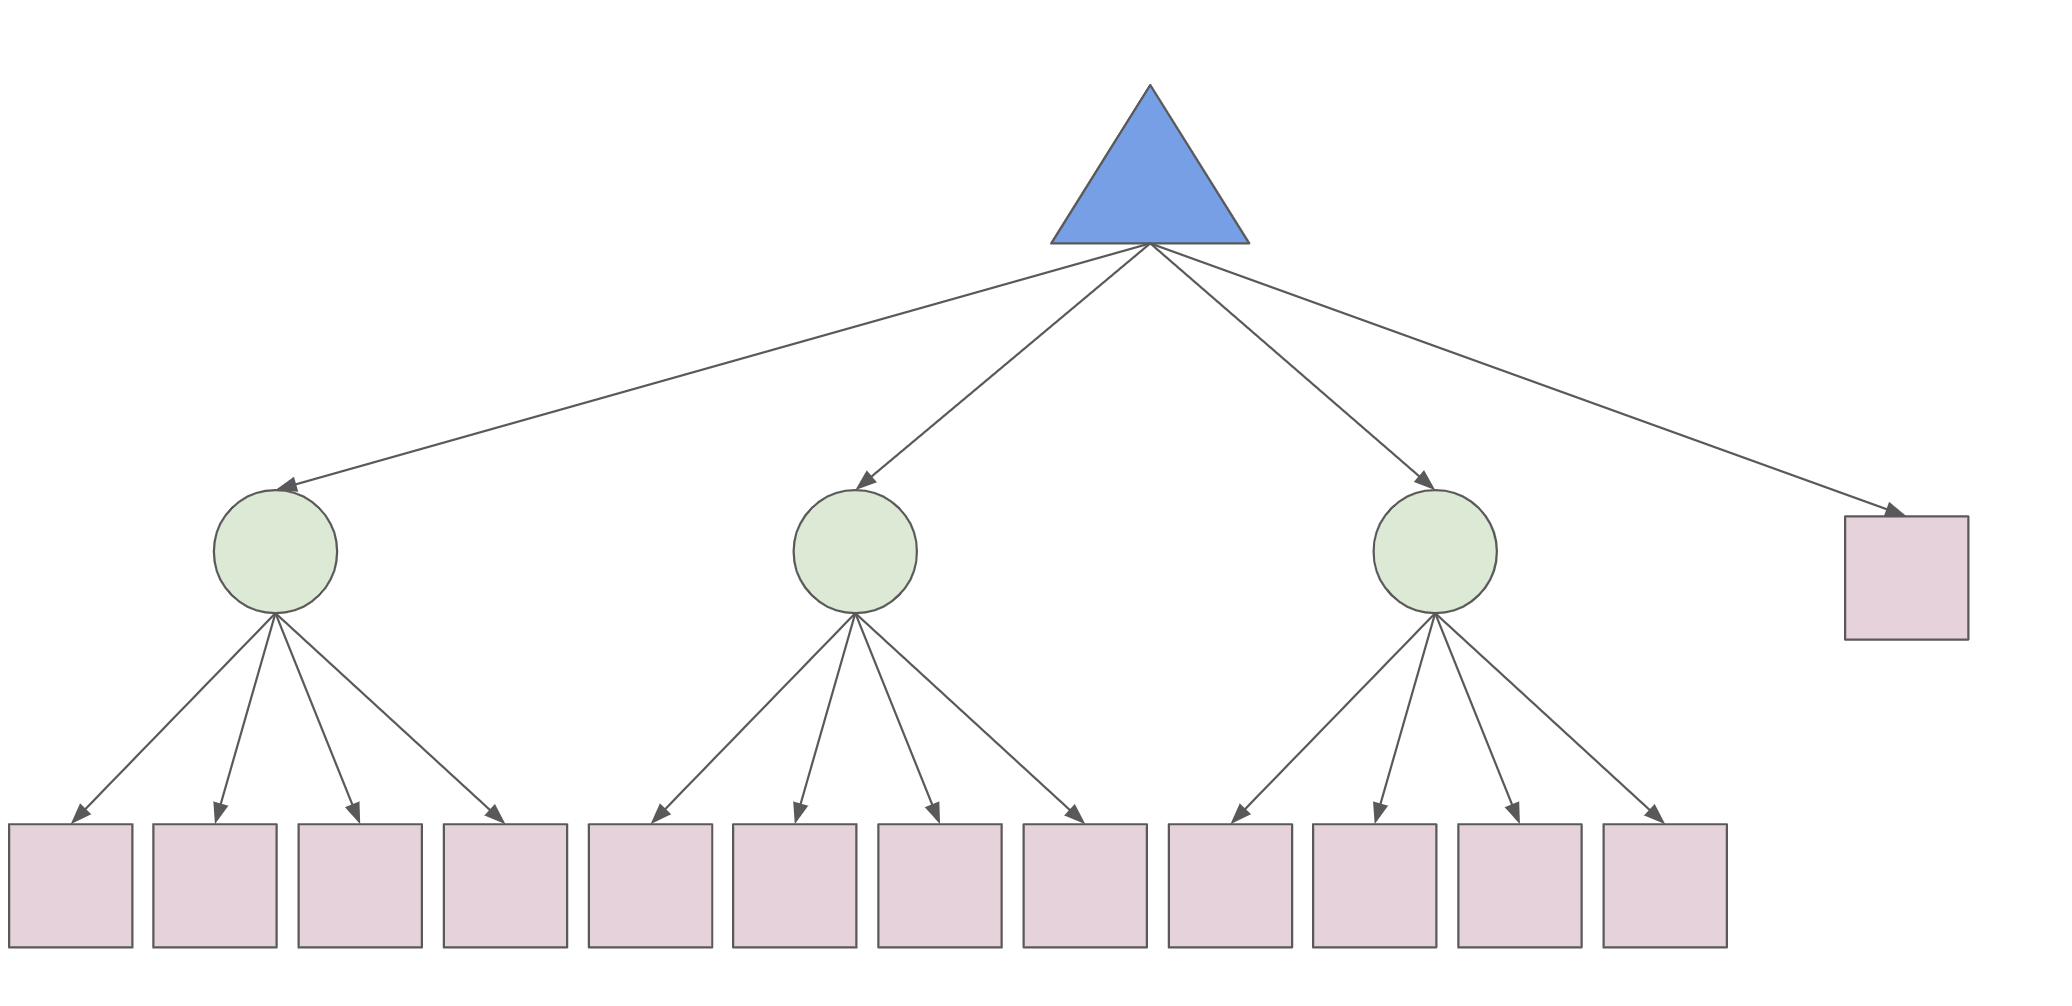
\includegraphics[width=0.7\textwidth]{figures/q1_graph_noblank.png}
\label{fig:expectimaxempty}
\end{center}

\end{subquestion}
\newpage
\begin{subquestion}[7]
Given a starting roll (1,2,4) (corresponding to the outcomes of die rolls 1, 2, and 3 respectively), what move should you take? Fill in the values of the expectimax tree below to justify your answer.

\begin{center}
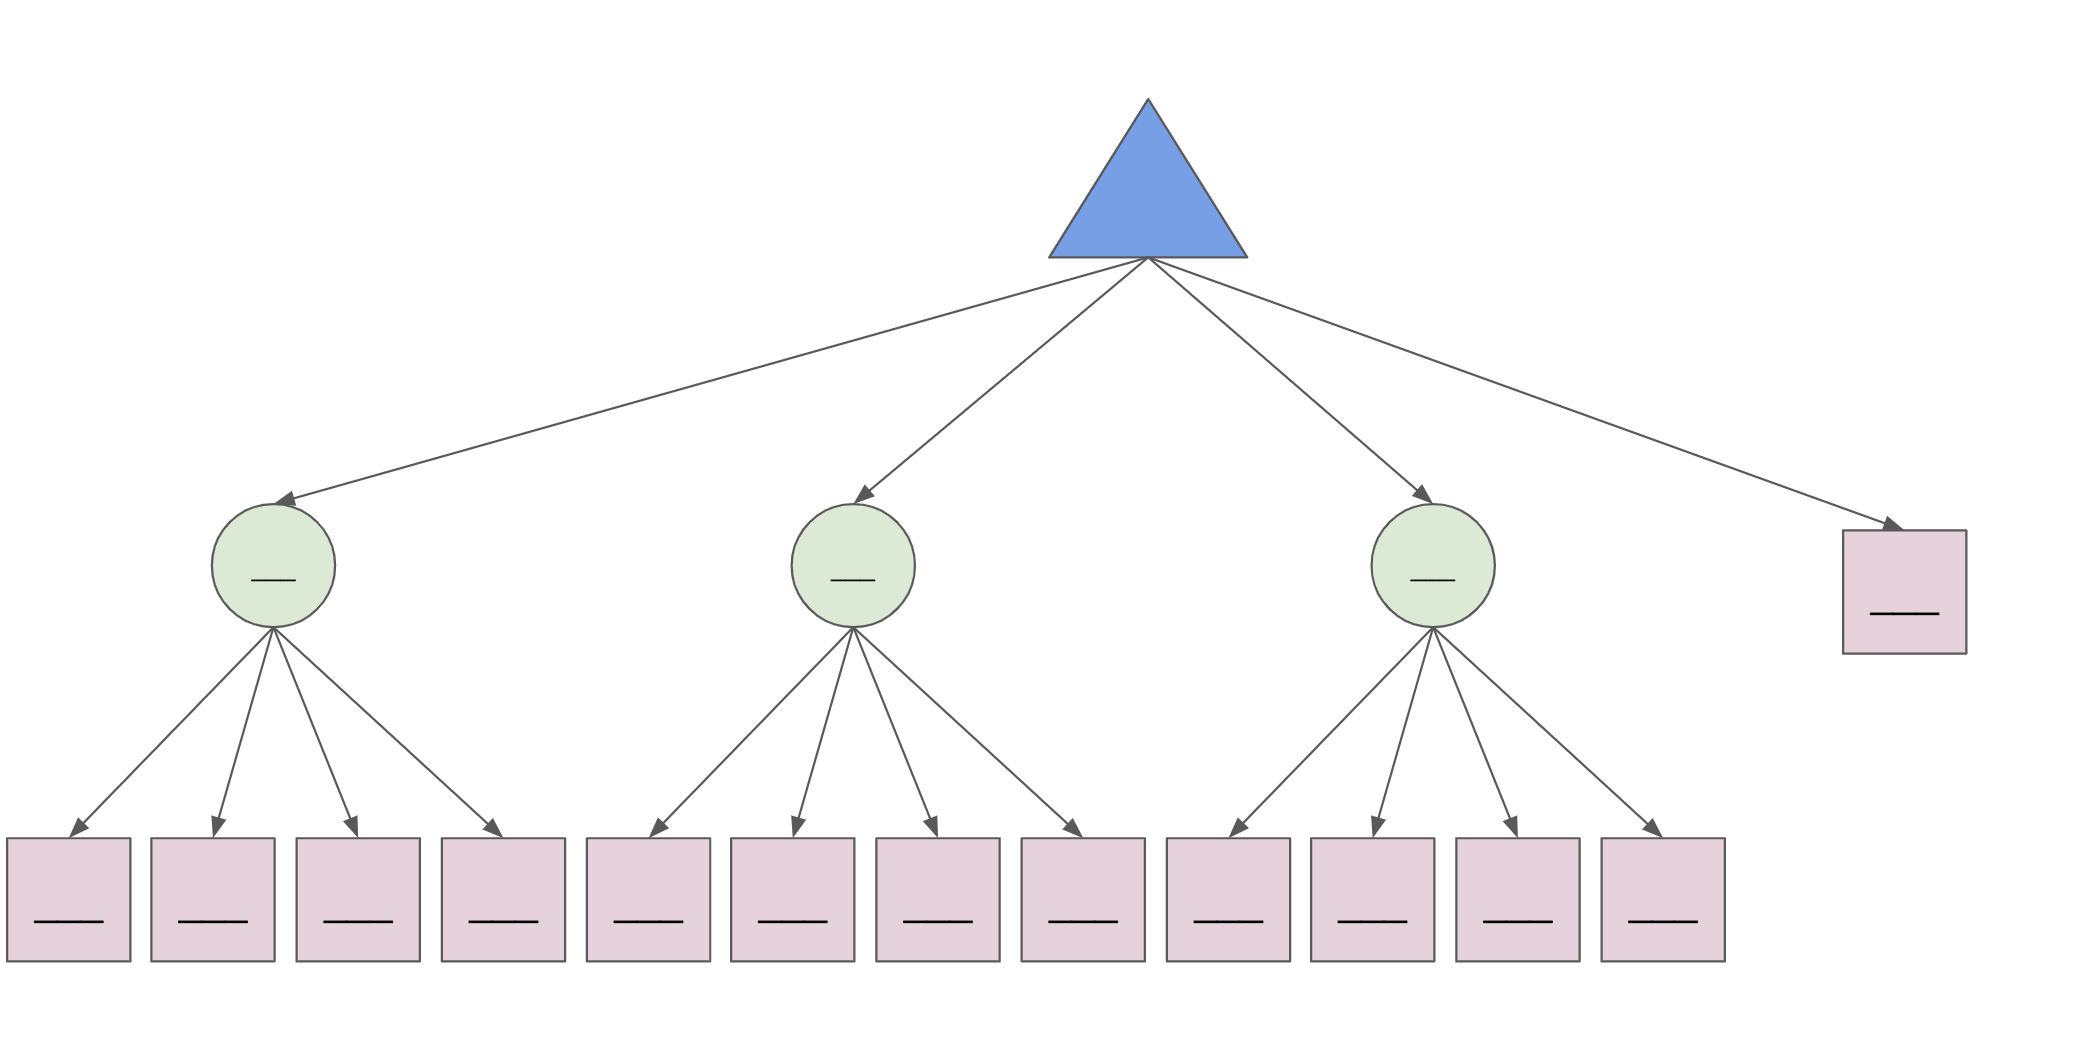
\includegraphics[width=0.7\textwidth]{figures/q1_graph.png}
\label{fig:expectimaxempty}
\end{center}

\end{subquestion}
 
\end{question}
\newpage
Now suppose the human player does not understand how to play the game, and as a result, they choose any action with uniform probability, regardless of the initial roll. Moreover, we assume that the human's choice will be carried out by a "somewhat helpful" robot called Albertbot: given a configuration of dice and the desired action from the human, this robot either actually implements the human's action (with probability $1-p$) or overrides it with a `no reroll' action (with probability $p > 0$). If the human action is already `no reroll', then the robot does not interfere.


\begin{question}
Given a particular Yahtzee roll $roll$, Let $A$, $B$, $C$ and $D$ be the expected reward of performing actions `reroll die 1', `reroll die 2', `reroll die 3', and `no reroll', respectively.




\begin{subquestion}[3]
Which of the following trees best represents the expectimax tree, after accounting for the presence of the Albertbot?

\mcqs 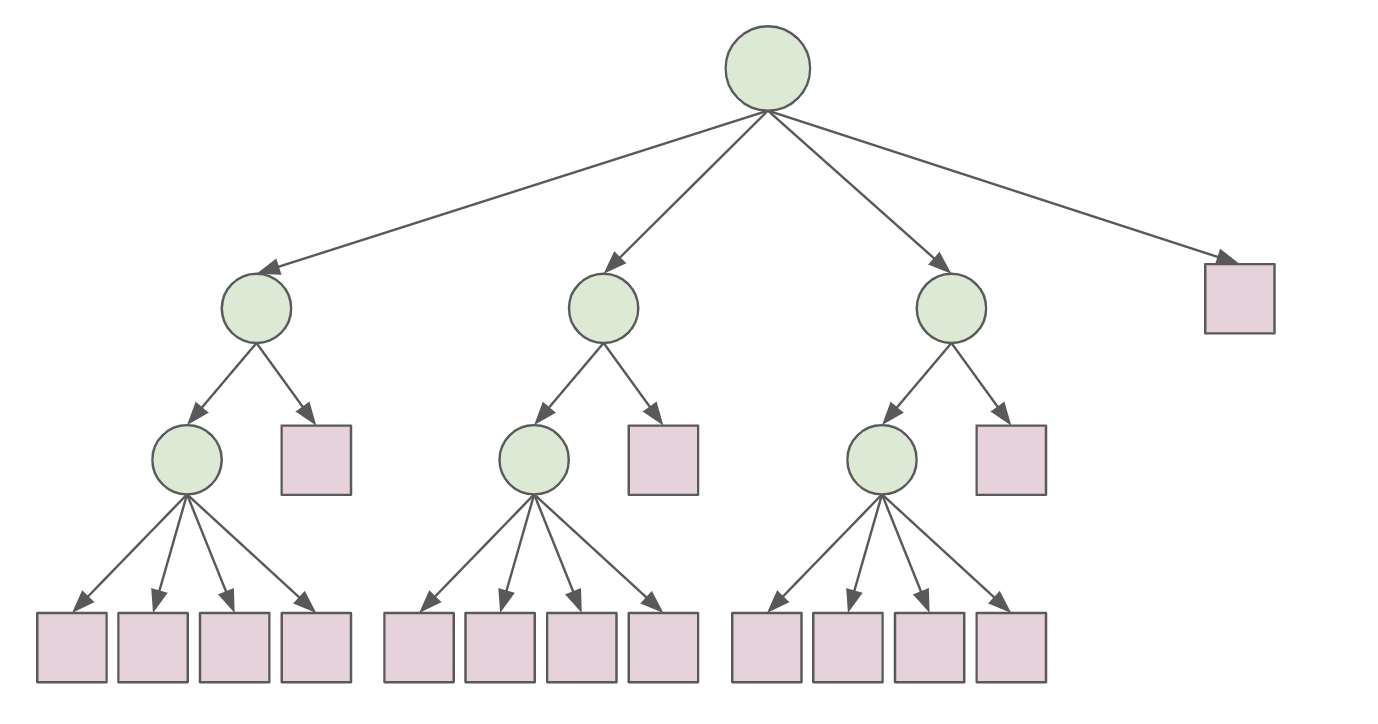
\includegraphics[width=250pt]{figures/q1_bot_a.png}

\mcqb 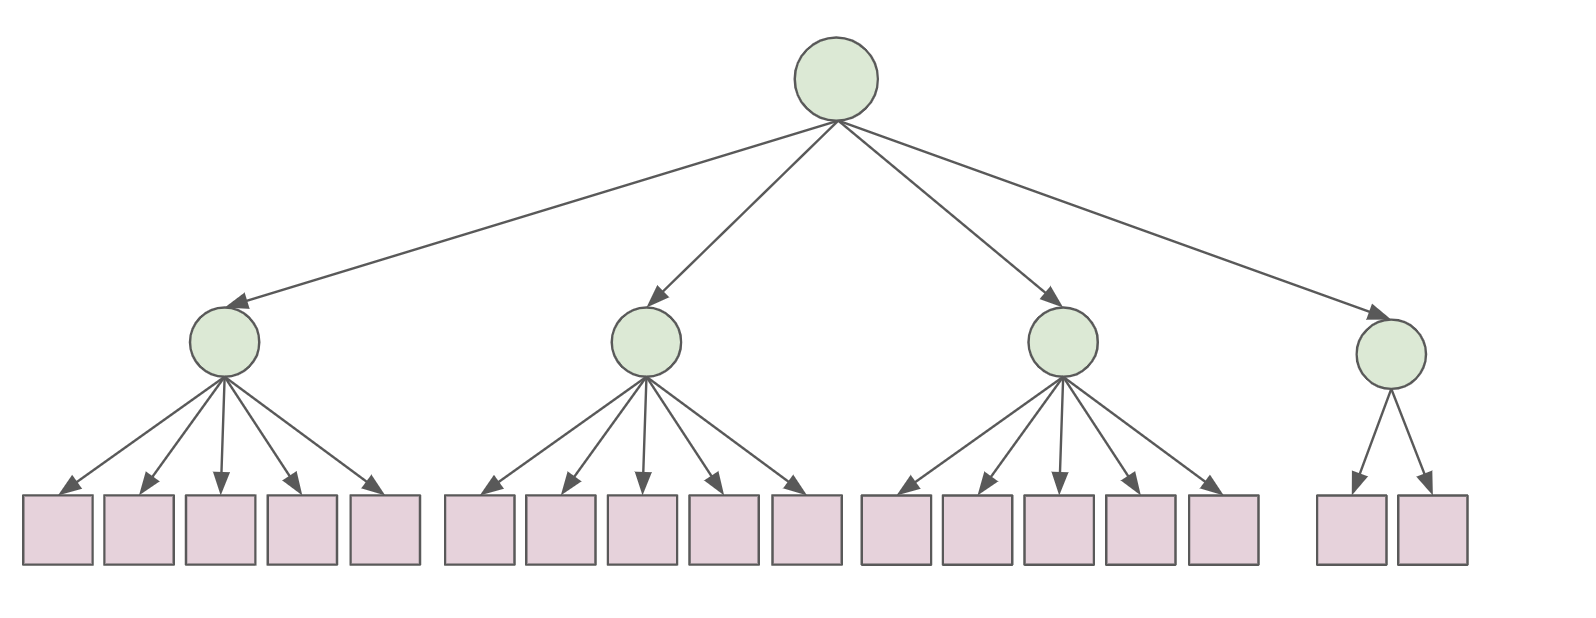
\includegraphics[width=250pt]{figures/q1_bot_b.png} 

\mcqb 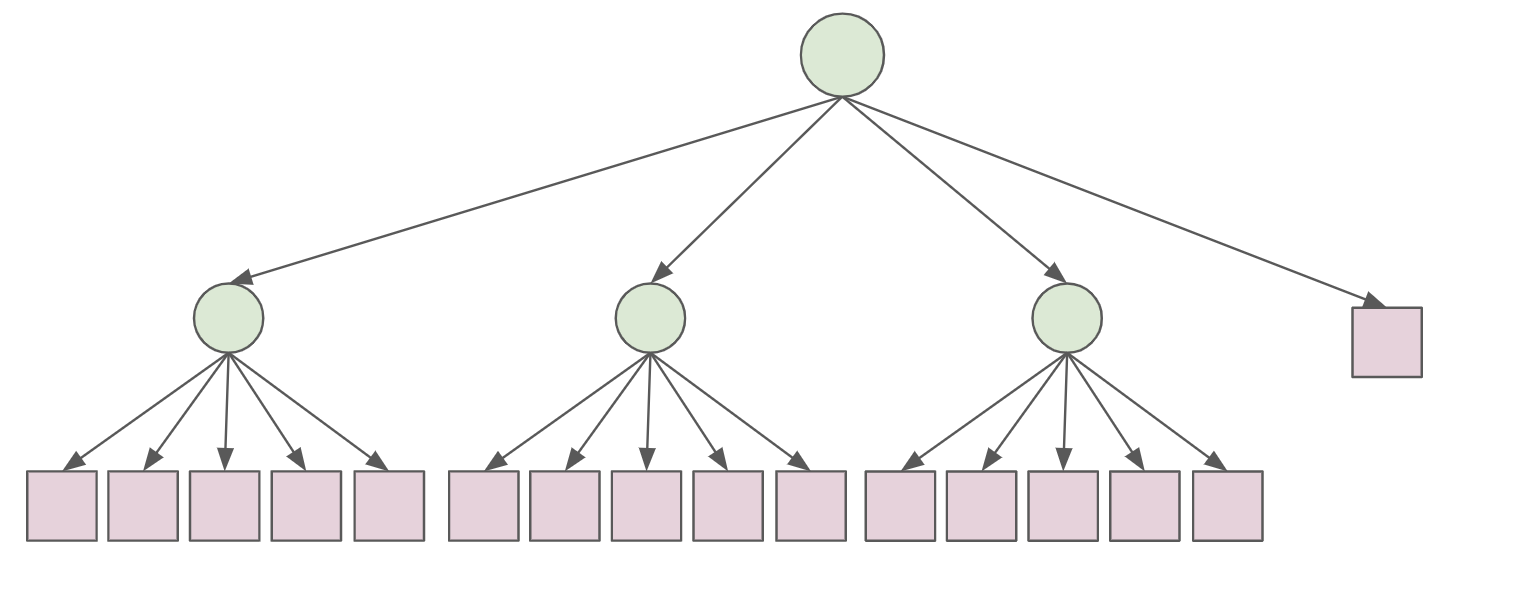
\includegraphics[width=250pt]{figures/q1_bot_c.png}

\mcqb 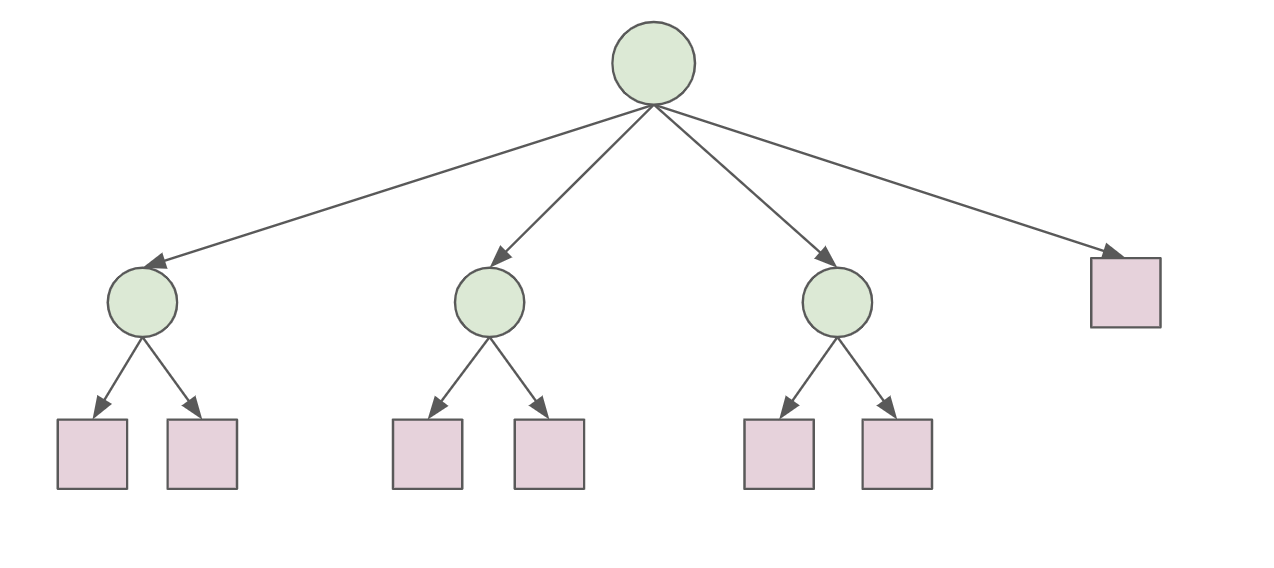
\includegraphics[width=250pt]{figures/q1_bot_d.png}
\\
\mcqb None of the above.
\\


\end{subquestion}




\newpage
\begin{subquestion}[5]
Express $R_H$ and $R_{AH}$ in terms of $A$, $B$, $C$ and $D$, where:
\begin{itemize}
    \item $R_H$ is the expected reward for the human acting {\em without} Albertbot's help.
    \item $R_{AH}$ is the expected reward for the human acting {\em with} Albertbot's help.
\end{itemize}
\textbf{Show all steps of your work} and \textbf{write your expression into the form of $X + Y p$}, where $X$ and $Y$ are expressions that contain $A$, $B$, $C$ and $D$ but not $p$. \\

$R_H =$

$R_{AH} =$

\end{subquestion}

\begin{subquestion}[5]
What is the condition for our Albertbot to strictly increase expected reward? Write the condition above using only $A, B, C, D, >$.

\end{subquestion}{}

\begin{subquestion}[2]
In one sentence, please describe the situation when the condition above is true.

\end{subquestion}



\end{question}


\newpage
\begin{question}[]
Your friend Diana argues that a helpful robot should not only override the human player's ``reroll" choice with probability $p$ (and replace it with a ``no reroll"), but also override the human player's ``no reroll" choice with probability $p$ (and replace it with the outcome of selecting one of the 3 dice at random and rerolling that dice). Diana needs your help with drawing the new expectimax tree for the Dianabot.


\begin{subquestion}[5]
Draw the expectimax tree for Dianabot. You need to draw out the tree with all nodes in their correct shapes; you do not need to label any values in the tree. Hint: you can start by modifying the expectimax tree for the Albertbot.
\end{subquestion}

\newpage

\begin{subquestion}[5]
What is the expected reward for a random human player with Dianabot's assistance? Again, please \textbf{show all steps of your work} and \textbf{write your expression into the form of $X + Y p$}, where $X$ and $Y$ are expressions that contain $A$, $B$, $C$ and $D$ but not $p$.

$R_{DH} =$

\end{subquestion}

\begin{subquestion}[5]
Under what condition on A, B, C, D is the human better off using Dianabot rather than Albertbot?


\end{subquestion}{}



\end{question}





\end{problem}

\end{document}
